\section{Decorators}


\subsection{Decorators}
\begin{frame}
\frametitle{Decorators}
	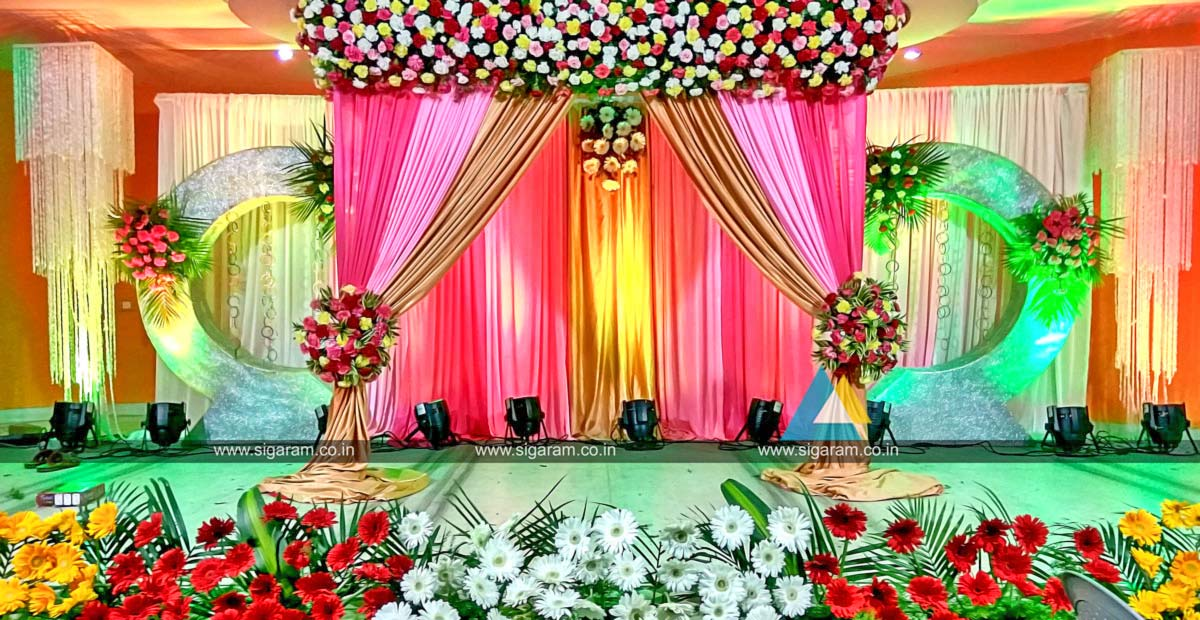
\includegraphics[width=0.9\textwidth]{img/decorators.jpg}
\end{frame}

\subsection{Decorators}
\begin{frame}
\frametitle{What is a Decorator}
\setlength{\epigraphwidth}{0.9\textwidth}
\epigraph{``A decorator is the name used for a software design pattern.
Decorators dynamically alter the functionality of a function, method, or class without having to directly use subclasses or change the source code of the function being decorated."}{--- https://wiki.python.org/moin/PythonDecorators}

\end{frame}

\subsection{Decorators}
\begin{frame}
\frametitle{A simpler explanation}
Decorators help to write code that is easier to write and read. It helps to avoid repeating "boilerplate code".

It's \emph{syntactic sugar}.
\end{frame}


\subsection{Expressions}
\begin{frame}[fragile]
\frametitle{Expression functions}
\begin{lstlisting}[style=pythoncode]
@qgsfunction(args='auto', group='Custom')
def sum(value1, value2, feature, parent):
    """
    Calculates the sum of the two parameters value1 and value2.
    <h2>Example usage:</h2>
    <ul>
      <li>my_sum(5, 8) -> 13</li>
      <li>my_sum("field1", "field2") -> 42</li>
    </ul>
    """
    return value1 + value2
\end{lstlisting}
\end{frame}

\subsection{Processing}
\begin{frame}
\frametitle{Processing}
	\begin{columns}[T] % contents are top vertically aligned
		\begin{column}[T]{7cm} % each column can also be its own environment
			\begin{itemize}
				\item Modular data processing pipelines
				\item Less effort to create the GUI
				\item But: A lot of boilerplate code
				\begin{itemize}
					\item Processing provider
					\item Methods for input and output definition
					\item Methods for help
					\item Method for the algorithm itself
				\end{itemize}
			\end{itemize}
		\end{column}
		\begin{column}[T]{3cm} % alternative top-align that's better for graphics
			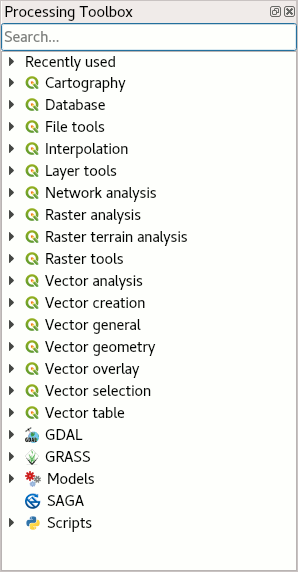
\includegraphics[height=7cm]{img/processing-toolbox.png}
		\end{column}
	\end{columns}
\end{frame}

\subsection{Processing}
\begin{frame}[fragile]
\frametitle{Processing Algorithm}
\begin{lstlisting}[style=pythoncode]
class GeoCoding(Algorithm):
	INPUT: 'INPUT'
	OUTPUT: 'OUTPUT'
	COLUMN_PREFIX: 'COLUMN_PREFIX'
	
	def name(self):
		return 'geocoding'
		
	def initAlgorithm(self, config=None):
		self.addParameter(
            QgsProcessingParameterFeatureSource(
                self.INPUT,
                self.tr('Address Layer')
            )
        )
	def displayName(self):
	def group(self):
	def shortHelpString(self):
	...
\end{lstlisting}
\end{frame}

\subsection{Processing}
\begin{frame}[fragile]
\frametitle{processing.alg decorator}
\begin{lstlisting}[style=pythoncode]
@alg(name="geocode", label=alg.tr("GeoCode"))
@alg.input(type=alg.SOURCE, name="INPUT", label="Adress layer")
@alg.input(type=alg.SINK, name="OUTPUT", label="Output layer")
def geocode(instance, parameters, context, feedback, inputs):
    """
    Geocode locations. Addresses in, points out.
    May produce multiple points for an address if ambiguous.
    """
	source = instance.parameterAsSource(parameters, "INPUT", context)
	(sink, dest\_id) = instance.parameterAsSink(parameters, "OUTPUT", context, source.fields(), QgsWkbTypes.Point, QgsCoordinateReferenceSystem(4326))

	GeoCoder.resolve(source, sink)
	
	return {"OUTPUT": dest\_id}
\end{lstlisting}
\end{frame}

\subsection{Processing}
\begin{frame}[fragile]
\frametitle{processing.alg decorator}
\begin{lstlisting}[style=pythoncode]
@alg(name="geocode", label=alg.tr("GeoCode"))
\end{lstlisting}

\end{frame}


\subsection{Validity checks}
\begin{frame}[fragile]
\frametitle{Validity checks}
\begin{lstlisting}[style=pythoncode]
@check.register(type=QgsAbstractValidityCheck.TypeLayoutCheck)
def layout_map_crs_choice_check(context, feedback):
	layout = context.layout
	results = []
	for i in layout.items():
		if isinstance(i, QgsLayoutItemMap) and i.crs().authid() == 'EPSG:3857':
			res = QgsValidityCheckResult()
			res.type = QgsValidityCheckResult.Warning
			res.title='Map projection is misleading'
			res.detailedDescription='The projection for the map item {} is set to <i>Web Mercator (EPSG:3857)</i> which misrepresents areas and shapes. Consider using an appropriate local projection instead.'.format(i.displayName())
			results.append(res)

		return results
\end{lstlisting}
\end{frame}
